\chapter{Characterization}
\graphicspath{{../gfx/chapter03/}{../plots/chapter03/}}


\section{The three-cell wire}

We choose a simple QCA system, the three-cell wire that we had already
introduced in Fig.~\ref{fig:short_wire}(b) in the first chapter, to investigate
general time-independent characteristics of QCA circuits. Specifically, we are
interested in how the polarization of one cell \emph{responds} to the
polarization of a second cell, and how cell polarizations depend on cell-cell
distance and inter-cell angle. For the three-cell wire we use a
nearest-neighbour Coulomb repulsion $V_1 = 40$ and the cell-cell distance is
$d/a = 2.2$, where $a$ is the edge length of the cell. Most of our calculations
will be at finite temperature, $T = 1$, and we will concentrate on horizontal
wires for now (meaning the inter-cell angle is $\theta = 0^{\circ}$). Both the
Coulomb energy scale $V_1$ and the temperature $T$ are in units of the hopping $t$,
with $t = 1$. For these parameters the bond approximation is valid, and we
employ it unless otherwise noted. We investigate systems both without compensation
charges $q = 0$, here the net cell charge is $-2e$, and with a compensation
charge of $q=\frac{1}{2}$, yielding charge-neutral cells.

\begin{figure}
  \center
  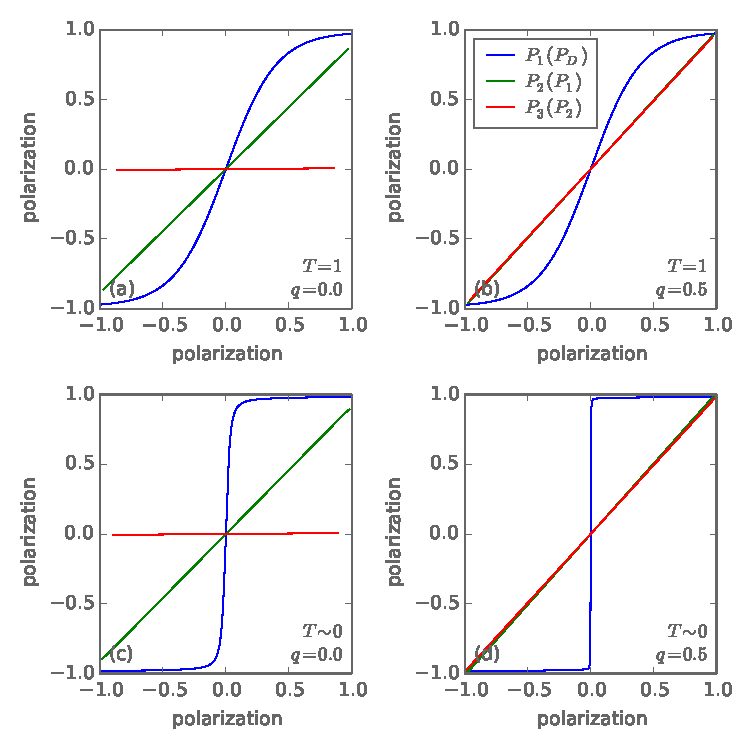
\includegraphics{three_cells_PP}
  \caption
  [The cell-cell polarization response]
  {
  The cell-cell polarization response. The response of the first cell with
  respect to the driver cell is non-linear and exhibits gain. In contrast, the
  response of the second cell with respect to the first cell, and similarly
  for the third with respect to the second, is linear and without gain. At zero
  temperature, the responses are generally improved, but the qualitative
  behaviour remains the same.
  }
  \label{fig:three_cells_PP}
\end{figure}

\begin{figure}
  \center
  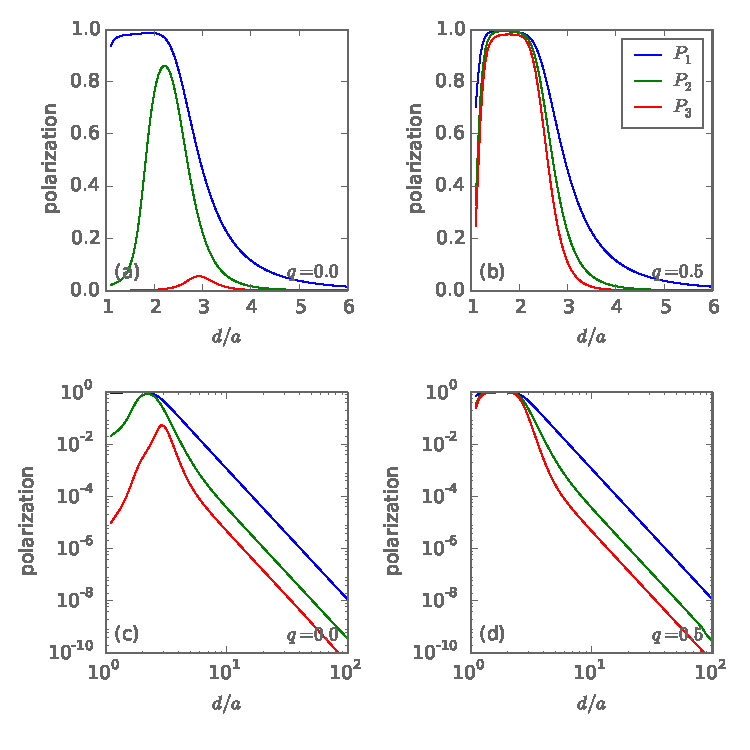
\includegraphics{three_cells_P_over_d}
  \caption
  [Cell polarization over cell-cell distance]
  {
  (a)(b)~Cell polarization over cell-cell distance. In the non-charge-neutral
  system ($q = 0$), due to charge buildup the maximum polarization for
  consecutive cells is at increasingly large cell-cell distances. Even at
  optimal distance the output polarization $P_3$ is very small. The output
  polarization is drastically improved for the charge-neutral system. Each cell
  attains its optimal polarization in the same range of cell-cell distances.
  (c)(d)~Cell polarization over very large cell-cell distances. For large
  distances $d/a > 10$ the polarizations settle into an universal long distance
  tail $d^{-5}$, independent of $q$ and as predicted by the Ising interaction
  $J$.
  }
  \label{fig:three_cells_P_over_d}
\end{figure}

The driver cell sets the input for the three-cell wire, with its
polarization $P_D$ taking values in the range $-1$ to $+1$. The three active
cells respond to the driver polarization. For our discussion, we define the
linear polarization response of cell $k$ with respect to cell $l$ as
%
\begin{equation}
  \label{eq:polarization_response}
  \chi_{kl} = \frac{\partial P_k}{\partial P_l}\big|_{P_l = 0} \, .
\end{equation}
%
Figure~\ref{fig:three_cells_PP}(a)~and~(b) show the polarization of the first cell
with respect to the driver cell, the polarization of the second cell with
respect to the first cell, and so on. For the first cell, the response is
non-linear and shows gain, therefore $\chi_{1D} > 1$. In contrast, the
polarization response between cells interior to the wire is linear and does not
exhibit gain, i.e.\ $\chi_{21} \le 1$ and $\chi_{32} \le 1$. Generally, the
polarization decreases monotonically from cell to cell, $|P_D| \ge |P_1| \ge
|P_2| \ge |P_3|$. In fact, for the $q=0$ system the polarization rapidly drops
to zero for the chosen parameters. The transmission is much improved for charge
neutral cells. In that case, the response is almost perfect, $\chi_{21} \sim
\chi_{32} \sim 1$.

It is worth pointing out that at zero temperature, where we have to use the
fixed-charge model rather than the inapplicable bond approximation, we observe
the same polarization response characteristics, as demonstrated in
Fig.~\ref{fig:three_cells_PP}(c)~and~(d). Quantitatively, for the same system
parameters the response is improved at zero temperature compared to $T=1$. For
example, the first cell's polarization response becomes a near-perfect step
function for the chosen parameters. But, importantly, it remains true that the
response inside the wire ($\chi_{21}, \chi_{32}$) is always linear and without
gain. Without compensation charges, the polarization of the third cell remains
zero even in the ground state, indicating that the cells are so closely spaced
that charge buildup pushes the electrons of the rightmost cell to the rightmost
edge.

In the literature, the non-linear nature of $P_1(P_D)$ has been noted
\cite{lent1993quantum} \cite{lent1993lines}, and the apparent gain $\chi_{1D} >
1$ has been invoked to argue for the robustness and fault-tolerance of the QCA
scheme. However, as our graph shows, this is only strictly true for the response
with respect to the static-charge driver cell. We believe that the picture where each cell
switches with gain with respect to its neighbours is an artefact of the
intercellular Hartree approximation (ICHA), which we had introduced in more
detail in Chapter \ref{ch:QCA_intro}. ICHA treats each cell individually in the
static charge mean field of the other cells in the system. In other words, in
the ICHA scheme, for each cell the rest of the system is approximated by an
effective driver cell.

We now fix the driver polarization at $P_D = 1$ and look at how the
polarizations of the active cells depend on the cell-cell distance $d/a$, see
Fig.~\ref{fig:three_cells_P_over_d}(a)~and~(b). At $d/a = 2$ all quantum dots in
the system are equally spaced, cells are placed a distance $a$ apart. At this
separation and smaller, our basic assumption of no inter-cell hopping breaks
down, as some dots in adjacent cells are now placed closer together than the
dots inside each cell. Thus $d/a \le 2$ is an unphysical limit. Conversely, at
very large cell-cell distances we expect the cells to become decoupled and
therefore all polarizations to be zero. Obviously, neither extreme limit is of
interest if our aim is to build functional QCA devices.

As already observed above, and in line with our intuition, polarizations
generally decrease from cell to cell as we go further away from the driver cell.
Without compensation charges ($q=0$) the polarization quickly falls off to very
small values, whereas for charge neutral cells ($q = \frac{1}{2}$) the situation
is much improved. The graph shows that there is a cell-cell distance that yields
maximal polarization for each cell. For the $q=0$ system---non-charge-neutral
cells---the optimal distance increases from cell to cell, due to charge buildup.
In contrast, with charge-neutral cells ($q=\frac{1}{2}$) the cell-cell distance
yielding optimal polarization does not change notably from cell to cell. In
fact, here a range of distances gives very good polarizations, as the
polarization saturates at values close to $P = 1$. Outside of this plateau
region cell polarizations still fall off quickly towards zero, for example for
cell-cell distances $d/a \gtrsim 3$. Of course, for a wire what really matters
is the output polarization. For the chosen parameters, this calculation
demonstrates that for a $q=0$ system we should choose $d/a \sim 2.9$. For
$q=\frac{1}{2}$ the range $d/a \sim 1.3 \ldots 2.3$ gives the best output
polarization. Worryingly, this range is very close to the lower, unphysical
limit!

Especially for the non-charge-neutral system, it is beneficial to allow for
different distances between different adjacent cells along the wire. Thus a
single $d/a$ parameter is replaced by $d_k/a$ with $k = 1,2,3$ for the
three-cell wire. Using a stochastic optimization scheme introduced by Sandvik
\emph{et al}.\ \cite{Sandvik2007}, we can optimize the $d_k/a$ for optimal
output polarization. We find that the output polarization is significantly
improved from $P_3 = 0.06$ for uniformly spaced cells to $P_3 = 0.15$ for cells
with individual cell-cell distances. Not surprisingly, cells are farther spaced
to the right (the output) and closer spaced to the left (the input). This is a
manifestation of charge buildup in the system. The situation is very similar for
longer wires and different parameters for non-charge-neutral wires. Of course,
non-uniformely spaced cells have implications for the directionality of
transport in a wire, which would have to be considered when designing QCA
circuitry. More generally, we should be able to optimize the functionality of
any given non-charge-neutral QCA layout by allowing for slightly adjustable cell
placement. We can do the same stochastic optimization for charge-neutral wires
($q=1/2$), but find that little is gained by allowing non-uniform cell-cell
distances. Looking at Fig.~\ref{fig:three_cells_P_over_d} this is really not
surprising at all, and simply a consequence of having no charge buildup in the
system. It should be emphasized how much better the output polarization is for
charge-neutral wires. At least for the chosen parameters, even very short wires
seem unrealistic for a non-charge-neutral system.

It is instructive to plot the polarizations over cell-cell distance up to very
large distances in a log-log graph as shown in
Fig.~\ref{fig:three_cells_P_over_d}(c)~and~(d). Even though large distances come
with extremely small polarizations that are not of practical interest, this
graph yields valuable insights into the nature of the interaction that mediates
the polarization. At distances $d/a > 10$ we see that the polarization settles
into an universal long range tail with $P(d) \sim d^{-5}$. This is consistent
with our understanding that the polarization is mediated by a
quadrupole-quadrupole interaction. For these large distances the polarization is
exactly the same for both the $q=0$ and the $q=\frac{1}{2}$ systems. Hence,
having non-charge-neutral cells does not actually alter the characteristics of
the cell-cell interaction. Instead, it suppresses the cell-cell interaction at
small distances. That is, charge repulsion competes with the quadrupole
interaction. The graph exactly confirms our analysis from Chapter
\ref{ch:approximations}. There, we had derived an approximate expression for the
mediating cell-cell interaction in the Ising picture, $J \sim d^{-5}$, to
leading order, and the derived $J$ was independent of $q$. At the time we had
seen that, in general, we can only map QCA to a modified Ising model with an
additional cell-cell interaction $J^{\prime}$, which does depend on $q$.
However, for the horizontal wire, $J^{\prime}$ vanishes and we are left with the
pure Ising model, and at large enough distances the behaviour of the
polarization is just as predicted. Of course, we are mostly interested in small
distances, where the polarization is relatively large. Here, the polarization
falls off faster than $d^{-5}$ and, remembering the derivation of $J$, we would
need to include higher order corrections in the multipole expansion to
accurately describe this behaviour. Even with higher order terms the Ising model
and its $J$ cannot, however, correctly reproduce the suppression of the
quadrupole interaction at short distances in the case of $q=0$.

\begin{figure}
  \center
  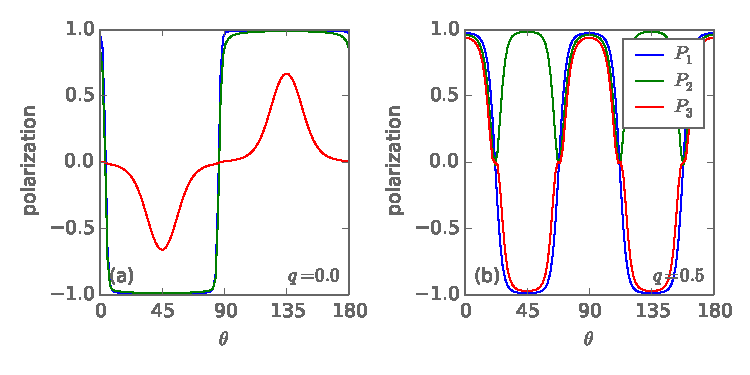
\includegraphics{three_cells_P_over_theta}
  \caption
  [Cell polarization over the inter-cell angle]
  {
  Cell polarization over the inter-cell angle. The charge-neutral system is
  invariant under rotations by $90^{\circ}$ and closely matches the behaviour
  predicted by the Ising $J$. At $45^{\circ}$ cell polarizations are
  alternating. For the non-charge-neutral system, the polarizations are
  predominantly set by the angle, and not by the driver polarization. The system
  is invariant under rotations by $180^{\circ}$, as predicted by the modified
  Ising $J^{\prime}$. In the non-charge-neutral case QCA does not work at all,
  except for horizontal or vertical wires.
  }
  \label{fig:three_cells_P_over_theta}
\end{figure}

From the discussion of the Ising model in Chapter \ref{ch:approximations}, we
already know that cell polarizations should change with the inter-cell angle.
The polarizations are mediated by the cell-cell interactions $J$ and
$J^{\prime}$, and specifically we had found $J \sim \cos{4 \theta}$, whereas
$J^{\prime} \sim \sin{2 \theta}$. We rotate the three-cell wire from a
horizontal configuration ($\theta = 0^{\circ}$) over diagonal ($\theta =
45^{\circ}$) to vertical ($\theta = 90^{\circ}$), and back to horizontal
($\theta = 180^{\circ}$), and look at the cell polarizations in the process.
Figure~\ref{fig:three_cells_P_over_theta}(b) shows the polarization as a function
of the angle for the charge-neutral system, where $J^{\prime} = 0$. Indeed, the
cell polarizations follow the behaviour predicted by $J$: they are rotationally
invariant under rotations by $90^{\circ}$ and peak at the angles $0^{\circ},
90^{\circ}$, and so on, where $J > 0$. At $45^{\circ}$, where $J < 0$, cell
polarizations are alternating, e.g.~$P_D \sim 1$, $P_1 \sim -1, P_2 \sim 1$, and
$P_3 \sim -1$. In between, for example at $\theta = 22.5^{\circ}$, $J = 0$ and
the polarization is zero accordingly. The wire can be used to transmit signals
in a range of about $20^{\circ}$ around $\theta = n \cdot 45^{\circ}$, where $n$
is an integer and the usable angle range depends on the chosen system
parameters. Of course, at $45^{\circ}$ we have to make sure to use an even
number of cells for transmission, as the signal will be inverted otherwise.
Conceivably, the nodes at $22.5^{\circ}, 67.5^{\circ}$, and so on could be used
to decouple closely spaced cells.

The situation is very different for non-charge-neutral systems, as shown in
Fig.~\ref{fig:three_cells_P_over_theta}(a). In this case, $J^{\prime} \ne 0$ and
we see that the polarization is actually predominantly set by $J^{\prime}$,
which is rotationally invariant under rotations by $180^{\circ}$. This is in
line with our derivation where we had found, to leading order, $J^{\prime} \sim
d^{-3}$, whereas $J \sim d^{-5}$, and thus, $J^{\prime}$ was expected to
dominate. The graph shows that the cell polarizations are much larger in
magnitude away from $0^{\circ}, 90^{\circ}$, and so on, where we know that the
system behaves as expected. In fact, the presented graph looks exactly the same
for $P_D = 1$ and $P_D = -1$, except for a small range of angles of about
$5^{\circ}$ around $\theta = n \cdot 90^{\circ}$, where the angle range again
depends on the chosen system parameters. In short, the cells' polarizations are
set by the inter-cell angle and not by the driver polarization. The importance
of charge neutrality had first emerged in our discussion of the Ising model.
Here we see this finding most impressively confirmed. The non-charge-neutral
system will never work as a QCA circuit unless all we want to do is build linear
chains of cells. Even in this case the system becomes very fragile with respect
to angular displacement. Thus, for QCA charge-neutral cells, $q=\frac{1}{2}$,
are absolutely essential. In the literature charge neutrality has usually been
assumed, either explicitly or implicitly, but as far as we know, no one else has
previously identified its crucial role.


\section{Workable parameters for QCA}

In the previous section we found charge-neutral cells to be essential for QCA.
Therefore we will from now on restrict ourselves to $q=\frac{1}{2}$ systems.
Additionally, we saw that in a line of cells the polarization is at best
preserved but generally decreases from cell to cell. There is no inter-cell
gain. If the cell-cell polarization response is less than ideal then the
polarization will eventually decrease to zero for a long line of cells,
rendering the wire non-functional. It is therefore important to identify a
parameter regime where the response is ideal or close-to-ideal as a prerequisite
for functional QCA circuits.

We use a cluster mean field approach beyond the single-site ICHA approximation
to calculate the polarizations of semi-infinite wires. A small cluster of active
cells is embedded in a large number of driver cells---the mean field---whose
polarization is set as the average of the active cells. The setup is illustrated
in Fig.~\ref{fig:semi_infinite_wire} for three active cells. Therefore, instead
of solving only the one-cell mean field Hamiltonian $H^{\mathrm{MF}}_k$
\eqref{eq:H_meanfield} introduced in section \ref{sec:basic_characterization},
as for the ICHA scheme, we solve a cluster mean field Hamiltonian
$H^{\mathrm{MF}}$, and instead of only using a single cell's polarization $P_k$,
the average of all active cells $\left< P_k \right>$ is used to set the mean
field $P_D$. The self-consistency condition then is
%
\begin{equation}
  P_D = \left< P_k \left( P_D \right) \right> \, .
\end{equation}
%
If we don't find a solution for the self-consistency condition for a given set
of parameters then only the trivial solution $P_D = 0$ remains. In this case no
self-consistent polarization exists.

We made a point of how problematic mean field approximations can be. Here we use
the approach to establish a \emph{lower bound} on workable parameters. In
principle, the number of active cells can be indefinitely increased and
properties of interest can be extrapolated to the thermodynamic limit; the
approximation is asymptotically correct. Of course, in practice the number of
active cells allowed by the available computer resources is actually quite small
and probably far from the asymptotic behaviour.

We have found that as few as ten driver cells on each side of the active cells
already look like an infinite wire. Adding more and more driver cells, the active
cells' polarizations quickly saturates, indicating that they don't ``see'' cells
farther away than ten cells. This also shows that in practice the interaction,
while beyond nearest-neighbour, is not extremely long-ranged. In the following
calculations we use 100 driver cells on each side of the active cells.

\begin{figure}
  \center
  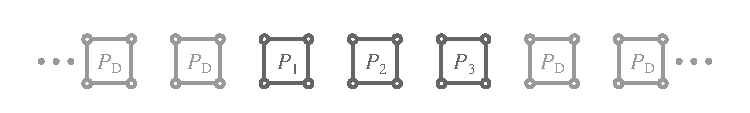
\includegraphics{semi_infinite_wire}
  \caption
  [The semi-infinite wire]
  {
  Semi-infinite wire. A small number of active cells is embedded in a large
  number of driver cells on both sides. The driver cells' polarization is
  determined self-consistently from the polarization of the active cells. This
  mean-field approach allows to establish a lower bound $V_{1\textrm{crit}}$ for workable
  nearest-neighbour Coulomb energies $V_1$.
  }
  \label{fig:semi_infinite_wire}
  
  \vspace*{0.75cm}
  
  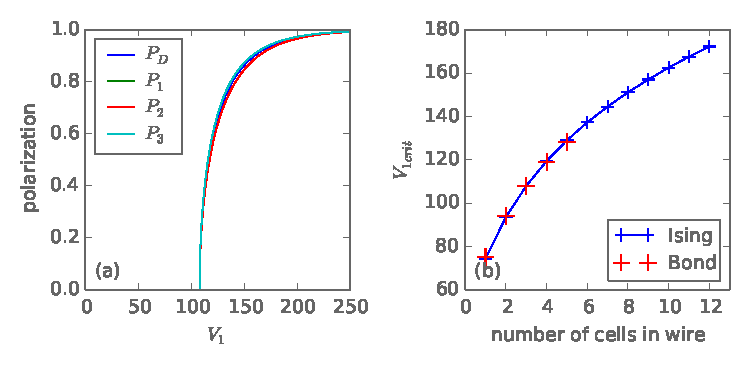
\includegraphics{critical_V1}
  \caption
  [Self-consistent polarization and critical $V_1$]
  {
  (a) Self-consistent polarization of a semi-infinite wire with three active cells.
  Below a critical $V_1$ no self-consistent solution exists and the polarization
  is zero throughout the wire. Above the critical $V_1$ the polarization grows
  quickly and saturates towards a perfectly polarized wire.
  (b) The critical $V_1$ as a function of the number of active cells in the
  semi-infinite wire: it grows monotonically and is expected to become infinite
  in the thermodynamic limit. For larger numbers of active cells the Ising model
  has to be used. Calculations with the bond model are included for comparison.
  }
  \label{fig:critical_V1}
\end{figure}

We now use a larger cell-cell distance $d/a = 3.0$ and a higher temperature $T =
2$, and calculate the self-consistent polarization with three active cells over
a wide range of values of $V_1$, shown in Fig.~\ref{fig:critical_V1}(a). We
observe a second-order phase transition at $V_{1\textrm{crit}}$. For $V_1 <
V_{1\textrm{crit}}$ no self-consistent solution with $P_D > 0 $ exists. This
regime is therefore inhibitive for QCA devices. Above the critical $V_1$ the
polarization rises very sharply and quickly saturates towards full polarization.
The presence of a phase transition is likely an artefact of the mean field
method. Still, the scale of the critical $V_1$ sheds light on what order of
magnitude to expect for a workable $V_1$. For our system, we find that $V_1
\gtrsim 150$ should yield large cell polarizations, and as before this is in
units of the hopping, with $t = 1$. For more favourably chosen parameters the
critical $V_1$ can also be much smaller. Table~\ref{tab:critical_V1} lists the
$V_{1\textrm{crit}}$ for a variety of different system parameters. In
particular, for the parameters used for the three-cell wire in the last section,
$T = 1$ and $d/a = 2.2$, the critical $V_1$ is only $V_{1\textrm{crit}} =
14.71$. The table also demonstrates that the critical $V_1$ grows very rapidly
for larger cell-cell distances. This is in line with what we had seen in
Fig.~\ref{fig:three_cells_P_over_d}(a)~and~(b), where we had plotted the cell
polarizations as a function of the cell-cell distance. In that graph, after a
plateau-like feature at small distances, the polarization had dropped off very
quickly with growing inter-cell spacing. Both observations emphasize that small
cell-cell distances are crucial, and, generally, we want distances as small as
possible while still satisfying our underlying physical assumptions, such as no
inter-cell hopping. Let us note that a graph qualitatively similar in appearance
to Fig.~\ref{fig:critical_V1}(a), obtained from single-cell ICHA calculations
for a seven-cell wire, has been reported in the literature previously
\cite{lent1993lines}. However, the reference's interpretation of the graph is
lacking. In particular, the significance and consequences of employing a mean
field scheme were not understood, and the critical values were therefore not
identified as lower boundaries, but taken at face value.

\begin{table}
  \center
  \begin{tabular}{c c r @{.} l p{0cm} c c r @{.} l}
    $T$ & $d/a$ & \multicolumn{2}{c}{$V_{1\textrm{crit}}$} & &
    $T$ & $d/a$ & \multicolumn{2}{c}{$V_{1\textrm{crit}}$} \\
    \hline 
    $1$ & $2.2$ & $ 14$&$71$ & &
    $2$ & $2.2$ & $ 25$&$99$ \\
    $1$ & $3.0$ & $ 55$&$10$ & &
    $2$ & $3.0$ & $107$&$90$ \\
    $1$ & $4.0$ & $230$&$24$ & &
    $2$ & $4.0$ & $459$&$87$ \\
  \end{tabular}
%  \begin{tabular}{c c r @{.} l}
%    $T$ & $d/a$ & \multicolumn{2}{c}{$V_{1\textrm{crit}}$} \\
%    \hline 
%    $1$ & $2.2$ & $ 14$&$71$ \\
%    $1$ & $3.0$ & $ 55$&$10$ \\
%    $1$ & $4.0$ & $230$&$24$ \\
%    $2$ & $2.2$ & $ 25$&$99$ \\
%    $2$ & $3.0$ & $107$&$90$ \\
%    $2$ & $4.0$ & $459$&$87$ \\
%  \end{tabular}
  \caption[Critical $V_1$ for different systems]{
  The critical $V_1$ obtained from bond model calculations with three active
  cells for a number of different systems.
  }
  \label{tab:critical_V1}
\end{table}

We now investigate how the critical $V_1$ changes with the number of active
cells and whether we can extrapolate to the thermodynamic limit, where the mean
field scheme becomes exact. Figure~\ref{fig:critical_V1}(b) traces
$V_{1\textrm{crit}}$ as the number of active cells is increased. With the more
accurate bond model only up to five cells are computationally feasible, and we
have therefore included calculations with the Ising model for up to twelve
active cells. For the chosen system parameters, the obtained values of the
critical $V_1$ are relatively large and the Ising model is therefore expected to
give sufficiently accurate results. Comparing the bond and Ising model in the
graph, we see that they indeed agree well. The bond model gives slightly larger
$V_{1\textrm{crit}}$ than the Ising model for one and two active cells, but for
four and five active cells the situation is reversed. Therefore, extrapolating
the trend, we believe that the Ising model slightly overestimates the critical
$V_1$ for larger numbers of active cells. This is in line with our observation
in section \ref{sec:validity_of_the_approximations} that the Ising model
generally underestimates the polarization. Most importantly, the graph shows
that the critical $V_1$ grows monotonically and substantially with an increasing
number of active cells. For the chosen parameters, the $V_{1\textrm{crit}}$ for
twelve active cells is more than twice the $V_{1\textrm{crit}}$ for only one
active cell. The critical $V_1$ grows more slowly for larger numbers of active
cells, but does not saturate, and there is no clear identifiable scaling
behaviour otherwise.  Therefore, we strongly suspect that the $V_1$ grows
indefinitely and becomes infinite in the thermodynamic limit. Conversely, for a
finite $V_1$ the polarization of the infinitely long wire will be zero.

We used a mean field semi-infinite wire to obtain a lower bound
$V_{1\textrm{crit}}$ for workable $V_1$ values. But we find that the
$V_{1\textrm{crit}}$ grows significantly with the number of active cells and in
fact eventually becomes infinite. The $V_{1\textrm{crit}}$ should still yield a
valid scale for finite size QCA systems, presumably of a size comparable to the
number of active cells in the mean field scheme, and certainly $V_1 <
V_{1\textrm{crit}}$ is a range where QCA is non-functional. More importantly
though, the fact that no finite thermodynamic limit exists implies that perfect
cell-cell response is impossible---the polarization along the wire will always
decreases monotonically---and that QCA systems are limited in size. We already
know from entropy arguments, laid out in section
\ref{sec:an_alternative_computing_paradigm}, that we cannot build infinitely
large QCA systems, so having a second size bound is not a show stopper. The
crucial question is whether we can achieve device units large enough in size to
do practical computations.

\begin{figure}
  \center
  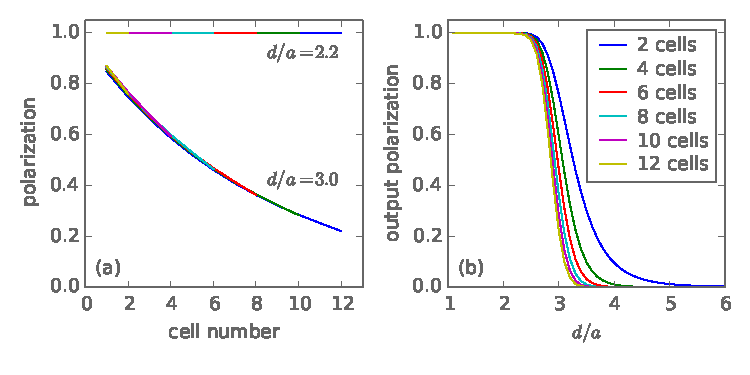
\includegraphics{wire_polarization}
  \caption
  [Cell polarizations along two- to twelve-cell wires]
  {
  (a) Cell polarizations of two-, four-, six-, eight-, ten-, and twelve-cell
  wires for two different cell-cell distances. Individual cell polarizations are
  hardly changed as the wire is made longer. The polarizations for the $d/a =
  2.2$ wire are essentially perfect.
  (b) Output polarization over cell-cell distance for different wires. The
  output polarization is perfect in a plateau-like region at small distances.
  For larger distances, $d/a \gtrsim 2.5$, the polarization very quickly drops
  to zero.
  }
  \label{fig:wire_polarization}

  \vspace*{1cm}
  
  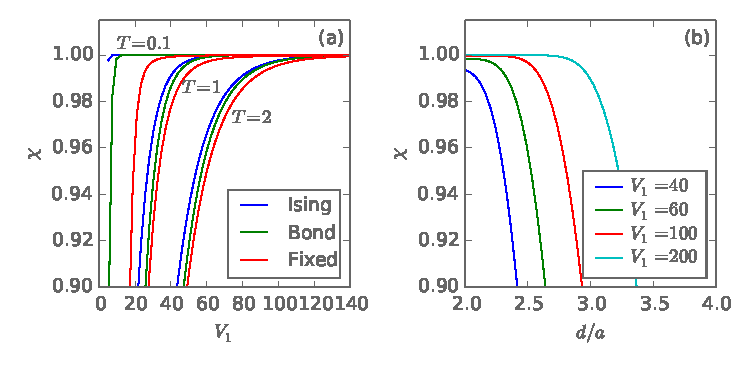
\includegraphics{chis}
  \caption
  [Cell-cell response over $V_1$ and cell-cell distance]
  {
  (a) The cell-cell response over the Coulomb energy $V_1$ at different
  temperatures and calculated with different models and wires. The fixed-charge
  wire slightly understimates the in-wire response, but is otherwise the most
  accurate model over the whole parameter range. For close to perfect response,
  $V_1 > V_{1min}$ is required with $V_{1min} \sim 120$, $V_{1min} \sim 60$, and
  $V_{1min} \sim 20$ for $T = 2$, $T = 1$, and $T = 0.1$, respectively.
  (b) The cell-cell response of the fixed-charge wire over cell-cell distance at
  $T = 1$. The distance range yielding close to perfect response increases with
  the Coulomb energy $V_1$. At $V_1 = 40$, close to perfect response is not
  achieved at any cell-cell distance.
  }
  \label{fig:chis}
  % TODO: too large
\end{figure}

To put into perspective the mean field $V_{1\textrm{crit}}$ values we found for
small QCA systems, we calculate the cell polarizations in two- to twelve-cell
wires at $V_1 = 200$---well above all the $V_{1\textrm{crit}}$ values in
Fig.~\ref{fig:critical_V1}(b)---and with a driver polarization of $P_D = 1$.
According to Fig.~\ref{fig:critical_V1}(a), which was calculated for three
active cells, at $V_1 = 200$ we should have a self-consistent average
polarization of $\left< P_k \right> = 0.97$ throughout the semi-infinite wire.
However, in an actual wire the cell polarizations are not constant, but drop off
quickly and are also much smaller, as shown in
Fig.~\ref{fig:wire_polarization}(a) in the $d/a = 3.0$ curve. For a six-cell
wire the output polarization is already less than half of the input
polarization, for twelve cells it is almost a fifth. The graph strongly suggests
that the polarization will continue to drop to zero for longer wires.  It
therefore becomes apparent that the mean field $V_{1\textrm{crit}}$ really does
set a lower boundary, and in practice significantly larger $V_1$ values are
necessary for functional QCA devices, even for relatively small systems.

Figure~\ref{fig:wire_polarization}(a) also includes cell polarizations for wires
with a cell-cell distance $d/a = 2.2$. For these systems,
Table~\ref{tab:critical_V1} lists $V_{1\textrm{crit}} = 25.99$, which was determined for
three active cells in a semi-infinite wire. An Ising model calculation with
twelve active cells yields $V_{1\textrm{crit}} \sim 45$, which likely overestimates the
critical $V_1$ and, for these small $V_1$ values, should really be taken as a
very rough guideline. At $V_1 = 200$ we are therefore almost an order of
magnitude larger than the critical $V_1$. At these shorter cell-cell distances
the cell polarizations are essentially perfect for all two- to twelve-cell
wires. When we zoom in, however, we find that the behaviour is qualitatively the
same as for the $d/a = 3.0$ wires: the polarizations still decrease
monotonically along the wire. But quantitatively the short cell-cell distance is
quite a different story. The polarizations fall off so slowly, that we can
reasonably expect to achieve sufficiently large output polarizations for very
long wires. To investigate the astounding quantitative difference between the
two systems, we again plot the polarization over cell-cell distance.
Figure~\ref{fig:wire_polarization}(b) shows the output polarization of two- to
twelve-cell wires. The graph looks qualitatively similar to
Fig.~\ref{fig:three_cells_P_over_d}(b) from the last section: for small
distances the output polarization is close to perfect in a plateau-like region,
but for $d/a \gtrsim 2.5$ rapidly drops to zero. And it drops increasingly
faster to zero for longer wires. Therefore, for large, functional QCA devices we
want to make sure we operate in the plateau-like regime at small distances.

The cell polarization curves for all two- to twelve-cell wires in
Fig.~\ref{fig:wire_polarization}(a) almost lie on top of each other, implying
that the polarizations of existing cells hardly change as the wire is made
longer by adding more cells to the right. We can directly inspect the cell
polarization responses along the wire $\chi_{i,i-1}$ and find that they are
almost constant, with the exception of the first cell which responds to the
driver cell and therefore behaves differently, and the last two cells, which
have slightly lower responses, due to edge effects. Additionally, the responses
are largely independent of the driver polarization, with the exception of the
response of the first cell, $\chi_{1D}$, of course, which we also find to
decrease for longer wires. The observed behaviour matches our intuition: we
know that the cell polarization responses interior to the wire are linear.
Symmetry suggests that the responses of cells far from the edges in a long wire
should be the same. Therefore, we are inspired to fit the cell polarization
curves to a simple physical model, 
%
\begin{equation}
  \label{eq:simple_model}
  P_k = \chi_e(P_D) \chi^k P_D \, .
\end{equation}
%
Here, $P_k$ is the polarization of cell $k$ in the wire, $\chi$ is the
polarization response which is assumed to be the same for all cells in the wire,
and $\chi_e(P_D)$ is the system response to the driver cell polarization $P_D$.
If the response to the driver cell was the same as for a regular cell, then we
would have $\chi_e(P_D) = 1$. We fit this model to the polarization curves, with
$P_D = 1$ fixed, and find that it works surprisingly well. Averaging over all
wires, we find $\chi_e = 0.999114(8)$ and $\chi = 0.999997(0)$ for $d/a=2.2$,
and $\chi_e = 0.97(4)$ and $\chi = 0.884(0)$ for $d/a = 3.0$. Similar to
$\chi_{1D}$, $\chi_e$ decreases slightly for longer wires, whereas $\chi$ is
almost perfectly constant (it increases very, very slightly with wire length).
If the model worked perfectly then both parameters would be the same for all
wires, but given that the model is so simple, we feel that it works reasonably
well, and over a range of system parameters. The assumption of constant cell
responses throughout the wire starts to break down for larger cell-cell
distances $d/a \gtrsim 4$, where the actual polarizations are already very small
for a majority of the cells.
% TODO: better numbers and _errors_ for chi_e and chi --- calculate the errors
% from the distribution of chi values

The graph in Fig.~\ref{fig:wire_polarization}(b) can be readily understood using
the simple model \eqref{eq:simple_model}. In the plateau region at small
cell-cell distances the cell responses interior to the wire are close to
perfect, $\chi \sim 1$. For larger distances, $\chi < 1$ and therefore the
polarization $P_k \sim \chi^k$ quickly falls off to zero for long wires. For
very long wires we expect the figure to resemble a step function. While $\chi$
does not depend on the driver polarization, it does depend on other system
parameters, like $d/a$ and $V_1$, and to be able to scale up to large system
sizes we want $\chi \sim 1$ and have to choose the parameters accordingly.

We can use the found values for $\chi_e$ and $\chi$ to roughly estimate how long
we can make the wires before the output polarization falls below a certain
threshold. More generally, this gives an approximate upper size for QCA devices
for the chosen system parameters. Averaging $\chi_e$ and $\chi$ over the two- to
twelve-cell wires, for the wire with $d/a = 3.0$ we find that the output
polarization drops below $0.1 P_D$ after $18$ cells. As the graph demonstrates the
output polarization already drops below $0.9 P_D$ before the first cell. In
contrast, with a cell-cell distance of $d/a = 2.2$, the output polarization is
above $0.9 P_D$ for up to $35,040$ cells, and above $0.1 P_D$ for up to a
staggering $771,988$ cells. These are very simple estimates that could likely be
improved, for example by extrapolating $\chi_e$ in a better way, but even if the
numbers are wrong by a factor of two or three, the improvement from $d/a = 3.0$
to $d/a = 2.2$ is most dramatic. For the smaller cell-cell distance the
potentially achievable system sizes are orders of magnitude larger than for the
larger cell spacing. With something like $30,000$ cells we can clearly build
practical circuit units that perform meaningful computations.

Our calculations show that the model $P_k \sim \chi^k$ is the right physical
picture for QCA wires, and by cranking up the system's parameters
we will be able to push the response increasingly close to perfect. Truly
perfect response, with $\chi = 1$, however, is not possible. As a consequence, in the
thermodynamic limit the polarization will always be zero. This picture agrees
with our observations of the critical $V_1$, which we had seen to grow to
infinity for infinitely large systems. Therefore, the polarization inside a wire
is never truly constant, but always decreases, if very slowly. The picture of
constantly and fully polarized QCA systems employed in the literature is
qualitatively wrong. Of course, by choosing the right system parameters and
making $\chi$ large enough, we can, in principle, achieve system sizes that
should be more than sufficient to build practical device units. 

We have shown explicitly that a set of parameters exists where QCA works well up
to large system sizes: $V_1/t = 200, T/t = 2$, and $d/a = 2.2$. These parameters
are rather extreme and were partly chosen so that the Ising approximation is
valid, which allowed us to do calculations with wires of up to twelve cells. For
practical QCA implementations, however, it is important to identify minimal
workable parameters, specifically a minimal $V_1$ and a range of cell-cell
distances at a given temperature. The mean field $V_{1\textrm{crit}}$ is an indicative
value, of course, but we have just seen that it is ultimately not very reliable.
Following the simple model \eqref{eq:simple_model}, we can calculate the
cell-cell response $\chi$ in short wires with more accurate models over wide
parameter ranges and use this short-wire response as an estimate for the
response inside very long wires. According to the model, those responses should
be exactly the same. In practice, there are small differences due to more
pronounced edge effects in short wires.

Figure~\ref{fig:chis}(a) shows the cell-cell response over $V_1$ for three
different temperatures and for three different wires and models. Specifically,
the $\chi$ is calculated as the response of the sixth cell in an eight-cell wire
with the Ising model, as the response of the third cell in a four-cell wire with
the bond model, and as the response of the second cell in a two-cell wire with
the fixed-charge model, which is the most accurate model of the three. If the
assumption of constant $\chi$ for all wires is true, and if we are additionally
in a parameter regime where all three approximations become exact, then all
three curves should agree. The presented calculation uses a cell-cell distance
$d/a = 2.2$ and very small driver cell polarizations $P_D = 0.01$. The latter is
chosen so that cell polarizations do not saturate, $P_k < 1$, over the whole
parameter range.

For all three temperatures, the responses of the Ising, bond, and fixed-charge
wires all agree at large enough $V_1$, where we find $\chi \sim 1$.
Concentrating on the $T = 2$ curves, we see that bond and Ising agree for $V_1
\gtrsim 100$---where the Ising model becomes accurate---and their responses
become close to perfect around $V_1 \sim 120$. In contrast, the fixed-charge
$\chi$ is slightly smaller and only achieves $\chi \sim 1$ around $V_1 \sim
140$. In this regime, the bond and Ising model are both accurate, and the
difference between those two models' $\chi$ and the fixed-charge model's $\chi$
is due to edge effects of the shorter two-cell fixed-charge wire. Thus, while
the fixed-charge two-cell $\chi$ slightly underestimates the response in longer
wires, it clearly follows the trend of the other two models and can therefore be
used as a good estimate for the in-wire response in longer wires. At $T = 0.1$,
for example, bond and Ising model are no longer valid and give wrong results.
The fixed-charge model indicates that even at these small temperatures, perfect
response is only achieved for $V_1 > V_{1min}$ with $V_{1min} \sim 20$, and this
is also the minimum $V_1$ for any temperature. For $T = 1$ and $T = 2$, we find
$V_{1min} \sim 60$ and $V_{1min} \sim 120$, respectively.

We investigate how $\chi$ depends on the cell-cell distance.
Figure~\ref{fig:chis}(b) plots the fixed-charge two-wire response over the
cell-cell distance at $T = 1.0$ and for different values of $V_1$. Clearly, the
cell-cell distance range yielding $\chi \sim 1$ depends on the Coulomb energy
$V_1$: the larger $V_1$, the larger the distance range. In agreement with
Fig.~\ref{fig:chis}(a), the graph demonstrates that at $V_1 = 40$ close to
perfect response is not possible, even when going down to the lower physical
inter-cell distance limit $d/a = 2.0$. While $V_1 \sim 60$ is workable, $V_1
\sim 100$ seems like a comfortable regime where a range of cell-cell distances
$2.0 < d/a <2.5$ yield very good cell-cell responses. The figure remains
qualitatively unchanged at different temperatures. We find that the $\chi \sim
1$ distance range increase for lower temperatures, as can be expected. However,
at $T = 0.1$ and $V_1 = 20$ we cannot achieve close to perfect response at any
cell-cell distance.  Therefore, $V_{1min} \sim 20$ really is the lower limit for
operational QCA devices, at all temperatures. In summary, Fig.~\ref{fig:chis}
provides us with rough estimates for minimal workable parameters, and we have
used a loosely defined close-to-perfect polarization $\chi > 0.99$ to establish
them. As discussed above, how close to perfect is good enough depends on the
desired system sizes. However, we saw that for $\chi \lesssim 0.9$ only very
small systems are realistically achievable, and for $V_1 < V_{1min}$ the
response quickly drops below that mark.

We have used dimensionless parameters throughout. In the extended Hubbard model,
the energy scale is set by the hopping parameter, and we have chosen $t = 1$. We
use $V_1$ to characterize the Coulombic energies and found that very large
$V_1/t$ is a requirement for QCA. This Coulomb energy is set directly
by the cell size, $V_1 = 1/a$. Therefore, to achieve a very large
$V_1$, we need either very small cell sizes or a very small hopping $t$. Of
course, as the overlap integral the hopping $t$ also depends on the distance
between quantum dots, and thus the cell size. In a highly idealized system we
can assume the overlap integral to decay exponentially with dot-dot distance,
whereas the Coulomb interaction falls off as $1/r$. Therefore, in
principle, we can achieve the required large $V_1/t$ ratios simply by
making the QCA cells large enough. In practice, even if such an engineered
$V_1/t$ ratio were achievable, we might not gain much from it. An increasingly
small $t$ would ``freeze'' the system: dynamics would be very slow, greatly
reducing the usefulness for computation. The temperature is also in units of the
hopping parameter, and a small $t$ therefore potentially brings down the
tempterature to the cryogenic regime. Lastly, bringing down the overall energy
scales by reducing $t$ presumably would make the device more susceptible to
external perturbations in a less-than-perfect material system.

To put the minimal workable parameters we have found in a more tangible context,
we return to the atomic silicon quantum dots which we introduced in detail in
Section~\ref{sec:atomic_silicon_quantum_dots}. Even though this system is quite
different from our model---it uses six electrons per cell instead of two, and,
more importantly, is not charge neutral---it is close enough to get a rough idea
of what real world numbers might look like. Using \emph{ab initio} estimates
from reference \cite{pitters2011tunnel} for the hopping rate $t$ and the Coulomb
repulsion $V_1$ at various dot-dot distances, and fitting the data with the
simple assumptions $t \sim e^{-b a}$ and $V_1 \sim b a^{-1}$, where $b$ is a fit
parameter and $a$ the dot-dot separation, allows us to provide approximative
dot-dot distances for the $V_1/t$ ratios we have used. For example, to achieve
$V_1/t = 100$ would require a dot-dot distance and hence cell size of roughly $a
= 32 \mathring{\mathrm{A}}$. At $T/t = 1$, this corresponds to a temperature $T
= 4K$. We had found the absolute minimum $V_1$ to be $V_{1min}/t = 20$,
requiring $T/t \lesssim 0.1$. This would correspond to dot-dot distances $a = 22
\mathring{\mathrm{A}}$ and a temperature $T = 3 K$. While these are very rough
estimates, they still illustrate the challenge posed for experimental systems by
the large parameters required for QCA operation. On the silicon (100) surface
the dimer-dimer distance is $a = 3.84 \mathring{\mathrm{A}}$---the closest
possible spacing for two quantum dots. Therefore, the estimated dot separations
correspond to six to eight lattice spacings. The hopping constant becomes very
small and as a consequence the operational temperature moves to the single-digit
Kelvin regime. This is markedly different from the experiments and envisioned
setup of the group of Wolkow \emph{et al}., illustrated with a few examples in
Fig.~\ref{fig:silicon}, where dots are placed close to each other and room
temperature is used.


\section{The majority gate}

In the last section we identified a set of parameters for which the QCA approach
works very well up to large system sizes, specifically $T = 2, V_1 = 200, q =
1/2$, and $d/a = 2.2$, with, as always $t = 1$. For these parameters, we can use
the Ising model with good accuracy. It is instructive to look at more complex
QCA structures than the simple horizontal wire, and we pick the majority
gate---the single most important QCA logic device---as an example. The setup is
illustrated in Fig.~\ref{fig:gates}(a). The inputs are set with the driver cell
polarizations $I_1$, $I_2$, and $I_3$; the gate output is the polarization of
the rightmost cell, denoted by $O$. Each input lead consists of two active
cells, and similarly there are two cells for the output lead, for a total of
nine active cells. The polarizations of the input leads are understood to
``vote'' on the central device cell, with the majority polarization winning and
setting the final output.  We test the AND and OR functionality of the gate by
fixing one of its inputs to $-1$ and $1$, respectively, and we use $I_2$ as the
fixed input, for symmetry reasons.

\begin{figure}
  \center
  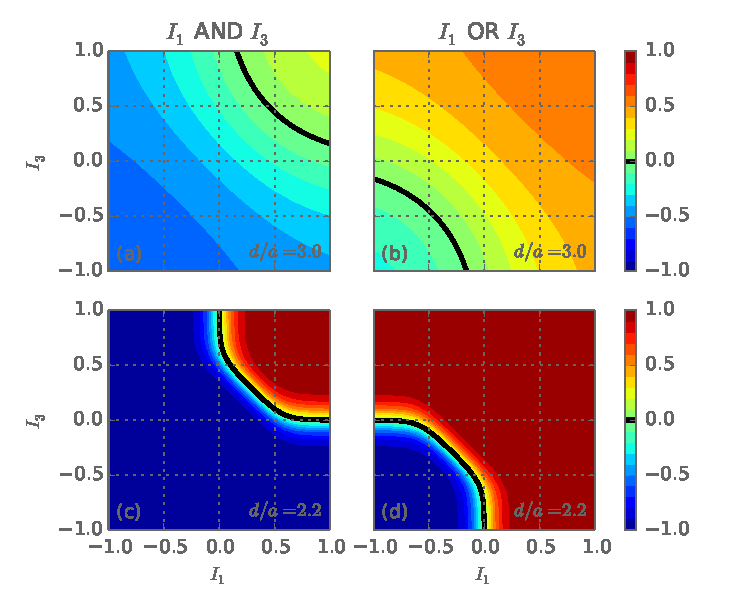
\includegraphics{majority_gate_contour}
  \caption
  [The majority gate]
  {
  Output polarization $O$ over input polarizations $I_1^{\prime}$ and
  $I_3^{\prime}$ of a majority gate in AND (with $I_2 = -1$) and OR (with $I_2 =
  1$) configuration. (a)(b) The majority gate with a cell-cell distance $d/a =
  2.2$. The gate correctly reproduces the AND and OR truth tables. The output
  polarization is linear with both input polarizations. (c)(d) The majority gate with
  a cell-cell distance $d/a = 2.6$---slightly outside the optimal parameter
  regime. The output polarization range becomes asymmetric with respect to the
  input polarizations. A non-zero input threshold is introduced.
  }
  \label{fig:majority_gate_contour}
\end{figure}

Figure~\ref{fig:majority_gate_contour}(a)~and~(b) show the output polarization as
a function of the two inputs for AND and OR gate configurations. Because the
response to driver cells is strongly non-linear, we do not plot directly against
$I_1$ and $I_3$, but use instead the polarizations $I_1^{\prime}$ and
$I_3^{\prime}$ of the cells right next to the driver cells, i.e.  the topmost
and bottommost active cells. This gives a more accurate picture for a gate in a
large circuit, far from the input driver cells. The gate implements the truth
table of $I_1 \land I_3$ and $I_1 \lor I_3$ correctly, for example $1 \land 1 =
1$ and $1 \land -1 = -1$. Unsurprisingly, the gate inherits the linear cell-cell
response, and therefore switches completely linearly with the input
polarizations. As an example, $0.5 \land 0.5 = 0.5$, and perfect output
polarization is only achieved for perfect input polarization. There is no input
threshold: any $I_{1,3} > 0$ is treated as a logic 1 state, and any $I_{1,3} <
0$ corresponds to logic 0. This is reflected by the fact that the zero contour
line exactly traces the outline of the upper right and lower left quadrant for
AND and OR gate, respectively.

We gain further insight into the characteristics of the QCA majority gate by
operating it slightly outside of the optimal parameter regime.
Figure~\ref{fig:majority_gate_contour}(c)~and~(d) show again the output
polarization for AND and OR gate configurations, but now at a larger cell-cell
distance $d/a = 2.6$. As can be expected, the output of the gate no longer spans
the whole polarization range from $-1$ to $+1$. The output range becomes
asymmetric with respect to the input range, for example $1 \land 1 \sim 0.8$,
but $-1 \land -1 \sim -1$. Similarly, we find that now there is a threshold
$I_{\textrm{th}} \sim 0.2$, where we require $\left| I_{1,3} \right| >
I_{\textrm{th}}$ so that the output is correct. Below the threshold, the gate
switches incorrectly, for example $0.1 \land 0.1 \sim - 0.1$. This asymmetry is
understood by considering the geometry of the gate. The cells of the input leads
$I_1$ and $I_3$ couple diagonally to the output lead and therefore induce a
polarization that is opposite to their own. Outside of the optimal parameter
regime, polarizations generally decrease from cell to cell, starting from the
driver cells. Thus, at larger cell-cell distances where the central cell is only
relatively weakly polarized, the influence of the more strongly polarized input
leads on the output lead becomes more important and consequently decreases the
overall output polarization and introduces a threshold. In this regime, if
instead of the symmetric $I_2$ one of the other two inputs, $I_1$ or $I_3$, is
used as the fixed input, then the output polarization also becomes asymmetric
with respect to switching the inputs.

Because QCA has no in-built directionality, different inputs are not decoupled
from each other. For example, the driver cell $I_3$ influences cells in the lead
of input $I_1$. This aspect is not directly captured by the graphs presented.
These are plotted against the effective cell polarizations $I_1^{\prime}$ and
$I_3^{\prime}$, which are directly or indirectly set by all three driver cell
polarizations $I_1$, $I_2$, and $I_3$. But as a consequence, the ranges of the
inputs $I_1^{\prime}$ and $I_3^{\prime}$ in the plots
\ref{fig:majority_gate_contour}(c)~and~(d) are truncated, simply because the
cells next to the driver cells never attain some polarization values. For
example in the AND configuration, if $I_3 = -1$, then we can never have
$I_1^{\prime} = 1$. We expect that for the design of larger circuits, consisting
of a network of gates and other elements, the relative magnitude of gate input
polarizations and the interference of various input driver settings need to be
considered. As a simple example, for the presented majority gate with
non-optimal parameters, input leads of different lengths would significantly
alter the behaviour.

Overall, we find that in the optimal parameter regime the majority gate works
well and functions as expected. The gate attains some undesirable
characteristics outside the optimal regime, such as an asymmetric output range
and non-zero input threshold, and in a real-world system these characteristics
might be exposed by fabrication imperfections and other perturbations.

% TODO: disucss that we could do optimize cell layouts classically; mention
% SSE montecarlo
